% !TeX spellcheck = it                                        

\documentclass[12pt,a4paper,openright,twoside]{report}
%openright: apre i capitoli a destra
%twoside: serve per fare un documento fronteretro


\usepackage[italian]{babel}
%\usepackage[latin1]{inputenc}
\usepackage[utf8]{inputenc}
\usepackage[T1]{fontenc} %aumenta il tempo di compilazione


%libreria per impostare il documento (headers & footers)
\usepackage{fancyhdr}


%libreria per avere l'indentazione all'inizio dei capitoli
\usepackage{indentfirst}

%libreria per personalizzare gli elenchi
\usepackage{enumitem}

%libreria per citare BibTex
\usepackage{cite}

%libreria per usasre il simbolo �
\usepackage[official]{eurosym}


%%%%%%%%%libreria per mostrare le etichette
%\usepackage{showkeys}

%libreria per inserire le note nelle tabelle
\usepackage{threeparttable}


%libreria per inserire grafici
\usepackage{graphicx}
\graphicspath{ {./img/} }


%libreria per inserire il codice
\usepackage{listings, xcolor}

\lstset{
    basicstyle=\ttfamily\footnotesize,
    breakatwhitespace=false,         
    breaklines=true
}



%%%%%%%%%%%%%%%%%%%%%%%%%%%%%%%%%%%%%%%%%libreria per utilizzare font particolari ad esempio  \textsc{}
%\usepackage{newlfont}


%%%%%%%%%%%%%%%%%%%%%%%%%%%%%%%%%%%%%%%%%librerie matematiche
%\usepackage{amssymb}
\usepackage{amsmath}
%\usepackage{latexsym}
%\usepackage{amsthm}


\oddsidemargin=30pt \evensidemargin=20pt%impostano i margini
\hyphenation{sil-la-ba-zio-ne pa-ren-te-si}%serve per la sillabazione: tra parentesi vanno inserite come nell'esempio le parole che latex non riesce a tagliare nel modo giusto andando a capo.


%%%%%%%%%%%%%%%%%%%%%%%%%%%%%%%%%%%%%%%%%comandi per l'impostazione della pagina, vedi il manuale della libreria fancyhdr per ulteriori delucidazioni
\pagestyle{fancy}\addtolength{\headwidth}{60pt}
\setlength{\headheight}{52pt}
\renewcommand{\chaptermark}[1]{\markboth{\thechapter.\ #1}{}}
\renewcommand{\sectionmark}[1]{\markright{\thesection \ #1}{}}
\rhead[\fancyplain{}{\bfseries\leftmark}]{\fancyplain{}{\bfseries\thepage}}
\cfoot{}


\linespread{1.3}    %imposta l'interlinea


%%%%%%%%%%%%%%%%%%%%%%%%%%%%%%%%%%%%%%%%%definisce nuovi comandi




\textwidth=450pt\oddsidemargin=0pt
\begin{document}

%scrivo il frontespizio
\begin{titlepage}
\begin{center}

{{\Large{\textsc{Alma Mater Studiorum $\cdot$ Universit\`a di
Bologna }}}}

%inserisce le 2 righe orizzontali
\rule[0.1cm]{15.8cm}{0.1mm}
\rule[0.5cm]{15.8cm}{0.6mm}

{\small{\bf SCUOLA DI SCIENZE\\
Corso di Laurea in Informatica }}
\end{center}
\vspace{15mm}
\begin{center}
{\LARGE{\bf Analisi Statica }}\\
\vspace{3mm}
{\LARGE{\bf di Smart Contract in Ethereum:}}\\
\vspace{3mm}
{\LARGE{\bf Stimare i Consumi di Gas }}\\
\end{center}
\vspace{40mm}

  

\par
\noindent
\begin{minipage}[t]{0.47\textwidth}
{\large{\bf Relatore:\\
Chiar.mo Prof.\\
Ugo Dal Lago}}
\end{minipage}
\hfill
\begin{minipage}[t]{0.47\textwidth}\raggedleft
{\large{\bf Presentata da:\\
Melania Ghelli}}
\end{minipage}

\vspace{20mm}

\begin{center}
{\large{\bf Sessione II\\%inserire il numero della sessione in cui ci si laurea
Anno Accademico 2018-2019 }}%inserire l'anno accademico a cui si � iscritti
\end{center}
\clearpage{\pagestyle{empty}\cleardoublepage}%non numera l'ultima pagina sinistra
\end{titlepage}

%scrivo la dedica
%\begin{titlepage}   %ambiente libero da vincoli


%\thispagestyle{empty}   %elimina il numero della pagina
%\topmargin=6.5cm 
%\raggedleft %incolonna la scrittura a destra
%\large  %aumenta la grandezza del carattere a 14pt
%\em %emfatizza (corsivo) il carattere

%Questa \`e la \textsc{Dedica}:\\
%ognuno pu\`o scrivere quello che vuole, \\
%anche nulla \ldots  %\ldots lascia tre puntini

%\newpage

%%%%%%%%%%%%%%%%%%%%%%%%%%%%%%%%%%%%%%%%
%\clearpage{\pagestyle{empty}\cleardoublepage}
%\end{titlepage}

\pagenumbering{roman}                   %serve per mettere i numeri romani

\tableofcontents                        %crea l'indice

%imposta l'intestazione di pagina
\rhead[\fancyplain{}{\bfseries\leftmark}]{\fancyplain{}{\bfseries\thepage}}
\lhead[\fancyplain{}{\bfseries\thepage}]{\fancyplain{}{\bfseries
INDICE}}

\listoffigures                     %crea l'elenco delle figure

%%%%%%%%%%%%%%%%%%%%%%%%%%%%%%%%%%%%%%%%%non numera l'ultima pagina sinistra
\clearpage{\pagestyle{empty}\cleardoublepage}

\listoftables                      %crea l'elenco delle tabelle

%%%%%%%%%%%%%%%%%%%%%%%%%%%%%%%%%%%%%%%%%non numera l'ultima pagina sinistra
\clearpage{\pagestyle{empty}\cleardoublepage}

\chapter*{Introduzione}            
\pagenumbering{arabic}

%%%%%%%%%%%%%%%%%%%%%%%%%%%%%%%%%%%%%%%%%imposta l'intestazione di pagina
\rhead[\fancyplain{}{\bfseries
INTRODUZIONE}]{\fancyplain{}{\bfseries\thepage}}
\lhead[\fancyplain{}{\bfseries\thepage}]{\fancyplain{}{\bfseries
INTRODUZIONE}}

%%%%%%%%%%%%%%%%%%%%%%%%%%%%%%%%%%%%%%%%%aggiunge la voce        Introduzione nell'indice
\addcontentsline{toc}{chapter}{Introduzione}


Le innovazioni tecnologiche introdotte negli ultimi decenni hanno rivoluzionato la nostra società. Il risultato che ne deriva è che numerosi settori stanno cambiando, muovendosi verso una realtà sempre più digitale. Se da una parte questo ha costituito un progresso, dall'altra ha creato nuove opportunità per i cybercriminali.\newline
Oggi il principale obiettivo della sicurezza informatica è proprio quello di trovare soluzioni adattabili alle nuove infrastrutture, come i sistemi IoT che si stanno diffondendo sempre di più. Con l'impiego di queste nuove tecnologie nell'industria i punti di accesso alla rete aziendale sono aumentati, moltiplicando la tipologia ed il numero di minacce. In questo contesto il rischio che si corre è maggiore, poichè legato alla violazione di dati sensibili o addirittura alla compromissione dei processi di produzione. %In questo scenario la cybersecurity è diventata una %disciplina di fondamentale importanza.
\newline
La blockchain nasce in questo contesto, riscuotendo un grande successo grazie al potenziale innovativo che porta con sé. Questa nuova tecnologia permette l'esecuzione di programmi in modo distribuito e sicuro, senza la necessitá di un ente centrale che faccia da garante. Il paradigma
trova applicazioni nei settori piú disparati, offrendo innovazione grazie alla
possibilitá di fare a meno di banche o istituzioni pubbliche.\newline
Ma in cosa consiste dal punto di vista informatico?
Blockchain, catena di blocchi.
Registro distibuito, organizzato in blocchi legati tra loro. Ad interagire con essa sono i miner, coloro che fisicamente realizzano le così dette transazioni. 
Qual è il ruolo del miner nello specifico??\newline
\newline
Grazie alla crittografia (sicurezza informatica comprende una serie di cose, tra cui la crittografia) è stato possibile implementare delle monete virtuali. Da questi studi si è arrivati poi a pensare al bitcoin, che è stato il primo esperimento condotto con successo.\newline
Ciò che indeboliva le crittovalute era il fatto di essere ''centralizzate'', cioè di passare per un ente che ne garantisse l'uso (una sorta di banca).\newline
La blockchain nasce come necessità di superare quest'ostacolo, perché finalmente introduce la possibilità di farne a meno.
Il primo esempio storico di moneta digitale si ha con il Bitcoin. Già da lui si parla di assenza di autorità centrale e rete distibuita - usando algoritmi proof-of-work. Questi permettono di raggiungere un consenso distribuito attraverso tutta la rete. E' il concetto chiave x capire come riusciamo ad evitare di affidarci ad un singolo ente es. Banca.\newline
Tra i sistemi nati grazie alla blockchain troviamo Ethereum, una piattaforma che mette a disposizione un linguaggio di programmazione di alto livello. Questo linguaggio puó essere utilizzato dagli utenti per implementare dei programmi, i così detti smart contract.\newline
In che cosa differisce dal Bitcoin?\newline
\newline
Gli smart contract possono essere eseguiti sulla rete di Ethereum solo al fronte di un pagamento anticipato. Per ragioni di sicurezza a ciascuna istruzione di basso livello è associato un costo monetario. Dunque eseguire un programma costerá tanto quante sono le istruzioni che lo compongono.
Il costo di ciascuna istruzione è espresso in termini di gas, una sorta di carburante che viene pagato in ether, la crittovaluta di Ethereum.
Dal momento che il gas viene pagato in anticipo, potrebbe accadere che l'esecuzione di un programma ecceda la quantitá messa a disposizione. In questi casi la computazione non giunge al termine, risultando nella perdita delle risorse investite dall'utente. Oltre a questo comportamento indesiderato l'esaurimento del gas disponibile puó avere conseguenze pericolose.
Un programma che non gestisce correttamente queste situazioni viene etichettato come vulnerabile. La conseguenza piú diretta è il blocco del contratto, che puó essere anche permanente. La pericolositá peró risiede nel fatto che questo tipo di programmi diventano un bersaglio facile per attacchi malevoli. Vedremo come queste vulnerabilitá possono essere sfruttate per ottenere
comportamenti dannosi per la rete.\newline
Dato il valore monetario associato agli smart contract il rischio che si corre in caso di attacchi informatici è una perdita di denaro. Per questo motivo è necessario individuare possibili criticitá nel codice prima della sua esecuzione. In questo contesto l'analisi statica dei programmi costituisce un potente
strumento di prevenzione.\newline
\newline
All'interno di questo elaborato ci concentreremo solo sulle tecniche di analisi dei consumi di gas. Poter conoscere a priori quest'informazione permetterebbe non solo un investimento adeguato da parte degli utenti, ma anche uno strumento di prevenzione da possibili attacchi.\newline
Attualmente non esistono strumenti in grado di calcolare con precisione la quantitá di gas richiesto durante una computazione. Cercheremo di capirne le ragioni ma soprattutto di individuare dei margini di miglioramento.\newline
\newline


%%%%%%%%%%%%%%%%%%%%%%%%%%%%%%%%%%%%%%%%%non numera l'ultima pagina sinistra
\clearpage{\pagestyle{empty}\cleardoublepage}

%%%%%%%%%%%%%%%%%%%%%%%%%%%%%%%%%%%%%%%%%imposta l'intestazione di pagina per i capitoli successivi
\rhead[\fancyplain{}{\leftmark}]{\fancyplain{}{\thepage}}
\lhead[\fancyplain{}{\thepage}]{\fancyplain{}{\rightmark}}

\chapter{Background}


Lo scopo di questo capitolo è quello di fornire una panoramica dei concetti chiave intorno ai quali si sviluppa l'elaborato.

\section{Blockchain}

Il termine Blockchain - in italiano ``catena di blocchi'' - identifica un registro distribuito e sicuro. In questo senso si può pensare alla blockchain come ad una struttura di dati simile ad una lista crescente, dove le informazioni sono raggruppate in blocchi collegati fra loro.\newline
Ciascun blocco codifica una sequenza di transazioni individuale, e viene concatenato a quello precedente seguendo un ordine cronologico. La concatenazione è irreversibile: ciascun nuovo blocco contiene la firma digitale di quello precedente. In questo modo, modificare un blocco implicherebbe l'invalidazione di tutta la catena successiva.\newline  
La peculiarità di questa struttura risiede nel fatto che sia condivisa: ogni nodo che compone la rete mantiene una copia del registro aggiornata. Per poter aggiungere un blocco è dunque necessario validare l'intera catena, ed ottenere un consenso da parte degli altri nodi della rete. Una volta ottenuto, il nuovo blocco viene trasmesso agli altri componenti in modo tale da aggiornare lo stato della blockchain.\newline
Il processo di validazione dei nuovi blocchi viene realizzato dai miner.
Il loro compito è quello di verificare le transazioni proposte e fare in modo che il nuovo blocco venga linkato alla blockchain. Per fare questo i miner sono chiamati a risolvere un algoritmo proof-of-work, un puzzle crittografico che richiede un significativo costo computazionale per essere risolto.\newline
Questo sistema permette di raggiungere il consenso senza la necessità di un'autorità centrale che faccia da garante. \'E il concetto chiave delle tecnologie basate su blockchain: la possibilità di implementare servizi sicuri senza appoggiarsi a banche, istituzioni pubbliche, ecc.\newline
\newline
Questa nuova tecnologia può essere integrata in diverse aree \cite{K1}, sebbene ad oggi il suo uso più conosciuto sia quello nei sistemi di pagamento che impiegano crittovalute.
Il dato non è poi così sorprendente: la prima blockchain nasce grazie a Satoshi Nakamoto assieme al Bitcoin \cite{K2}. In questo senso il Bitcoin è una
piattaforma di pagamenti, dove la catena di blocchi funge da storico di tutte le transazioni avvenute: una sorta di conto corrente condiviso.\newline

\section{Ethereum, gli Smart Contract e la EVM}

All'interno di quest'elaborato verrà presa in considerazione solo il network Ethereum, una piattaforma decentralizzata basata su una blockchain, che come Bitcoin possiede una propria valuta: l'\textit{ether}.\newline 
Diversamente da quanto vale per le altre crittovalute, Ethereum non è solo un network per lo scambio di moneta, ma un framework che permette l'esecuzione di programmi. Tali programmi prendono il nome di \textit{smart contract}, cioè ``contratti intelligenti''. Sebbene il nome possa suggerire una funzione ben precisa, questi programmi sono usati per computazioni general-purpose, permettendo quindi di realizzare un vasto numero di operazioni.\newline
Gli smart contract sono scritti in linguaggi ad alto livello; fra i vari (Serpent, Viper e LLL) quello più diffuso ad oggi è Solidity \cite{K3}. 
Tale linguaggio object-oriented è pensato solo per lo sviluppo di smart contract che, per poter girare nella rete, vengono poi tradotti in bytecode. Ciascun nodo di Ethereum infatti esegue localmente la Ethereum Virtual Machine, anche detta EVM, una macchina a stack in grado di eseguire un linguaggio di basso livello, ossia bytecode. Questo linguaggio è non tipato, e composto da un piccolo insieme di istruzioni.\newline 

\section{Il ruolo del gas}

Per \textit{gas} si intende l'unità di misura dello sforzo computazionale richiesto dalla EVM per eseguire ciascuna istruzione. Diremo quindi che eseguire uno smart contract costa una certa quantità di gas.\newline
Nello specifico ciascuna istruzione di basso livello ha associato un costo fisso in gas. Per calcolare quindi il consumo totale di un programma Solidity è necessario comprendere in quali istruzioni di basso livello verrà tradotto.\newline
I costi di alcune delle istruzioni EVM \cite{K4} sono riportati nella tabella \ref{tab:gas-costs}.
%(richiamo il nome della tabella utilizzando la label che ho messo sotto)

\begin{table}[h]                        %ambiente tabella
                                        %(serve per avere la legenda)
\begin{center}  %centra nella pagina la tabella

\begin{tabular}{p{5cm}rp{6cm}}  

\hline \hline   %inserisce due righe orizzontali
Istruzione & Costo & Descrizione\\   %& separa le colonne
\hline  %inserisce una riga orizzontale
\bf JUMPDEST & 1 & Indica la destinazione di un'istruzione JUMP\\
\bf POP & 2 & Rimuove un elemento dallo stack\\
\bf PUSHn & 3 & Inserisce un elemento di n byte nello stack\\
\bf ADD, SUB & 3 & Operatori aritmetici\\
\bf AND, OR, NOT, XOR, ISZERO, BYTE & 3 & Operatori logici\\
\bf MUL, DIV & 5 & Operatori aritmetici\\
\bf JUMP & 8 & Salto semplice senza condizione\\
\bf JUMP1 & 10 & Salto condizionale\\
\hline
\bf CALL & 700 & Chiama una transazione\\
\bf CALLVALUE & 9000 & Pagato per un argomento diverso da 0 dell'istruzione CALL\\
\bf SSTORE & 20000 & Salva una parola in memoria. Si paga quando il valore precedente è uguale a 0\\
\hline \hline
\end{tabular}

\caption[legenda elenco tabelle]{Costi espressi in gas di alcune istruzioni della EVM}\label{tab:gas-costs}
\end{center}
\end{table}

Il gas viene pagato in ether dagli utenti che intendono far eseguire una \textit{transazione}. Con transazione si intende l'azione di creare uno smart contract o di chiamarne delle funzioni e di pagare un miner per far eseguire la transazione stessa.\newline
Per fare in modo che la sua transazione venga scelta, un utente stabilisce la quantità di gas che è disposto a pagare per farla portare a termine. Il miner poi, in base a questo parametro, sceglie quali transazioni eseguire. \'E importante fornire un'adeguata somma: i miner, al termine della transazione, possono beneficiare dell'ether destinato all'acquisto di gas che è rimasto inutilizzato. Questo significa che gli smart contract con più probabilità di essere scelti sono quelli degli utenti disposti a pagare di più.\newline
La scelta adottata da Ethereum di far pagare i propri utenti non è triviale. Prima di tutto impedisce loro di sovraccaricare i miner di lavoro sfruttando il potere computazionale della rete. Inoltre scoraggia gli utenti a impiegare troppa memoria, una risorsa preziosa nelle tecnologie basate su blockchain. Infine limita il numero di computazioni eseguite dalla stessa transazione. Questo difende il network intero da attacchi malevoli come i DDoS: la finitezza delle transazioni fa sì che non si possa, ad esempio, far ciclare un programma infinitamente. Per poter disabilitare la rete anche solo per pochi minuti gli hacker dovrebbero pagare delle ingenti somme.\newline
Dal momento che il gas viene pagato anticipatamente, può succedere che durante la sua esecuzione un programma ecceda la quantità che ha a disposizione. Questo comportamento è  indesiderato, in quanto comporta spiacevoli conseguenze. La più immediata è il blocco della transazione: la computazione non giunge a termine, l'utente non ottiene il risultato desiderato e l'ether pagato per il gas va perso.\newline 
La conseguenza indiretta invece è il possibile blocco permanente dello smart contract. Quando durante l'esecuzione di una transazione un'istruzione richiede una quantità di gas superiore a quella disponibile, la EVM solleva un'eccezione di tipo \textit{out-of-gas} e interrompe la transazione. Qualora lo smart contract non preveda una gestione di questo tipo di eccezione resterà bloccato per sempre.\newline






%%%%%%%%%%%%%%%%%%%%%%%%%%%%%%%%%%%%%%%%%non numera l'ultima pagina sinistra
\clearpage{\pagestyle{empty}\cleardoublepage}

\chapter{Analisi Statica}

L'analisi statica è un processo di valutazione della correttezza dei programmi che rientra tra le tecniche di verifica del software. L'aggettivo \textit{statica} identifica una serie di controlli che possono essere effettuati sul codice prima della sua esecuzione. In questo si differenzia dall'analisi dinamica, una tecnica complementare che comprende quei controlli che vengono invece effettuati a runtime.\newline
\indent L'analisi statica solitamente è il primo controllo che viene effettuato sul codice durante lo sviluppo del programma.
% Perchè l'analisi statica non è common practice?
I vantaggi apportati da questo tipo di controllo del codice sono numerosi. I bug possono essere individuati per tempo, evitando comportamenti inaspettati da parte dei programmi. Inoltre, a seconda del tool utilizzato, è possibile migliorare il codice dal punto di vista della leggibilità, della strutturazione o della performance.\newline
\indent Tuttavia l'analisi statica resta una pratica poco diffusa tra gli sviluppatori \cite{johnson2013don}. Le principali cause sono da ricondursi agli output prodotti dai tool di analisi: l'elevato numero di warning così come la presenza di falsi positivi rendono gli strumenti meno affidabili. Oltre a questo, gran parte degli informatici afferma di non utilizzare questi tool di verifica a causa del sovraccarico di lavoro: spesso i ritmi aziendali così come la scarsa collaborazione dei team di sviluppo fanno sì che non ci siano i presupposti per dedicare spazio sufficiente all'analisi del codice.\newline


\section{Analisi Statica vs. Analisi Dinamica}

Per analisi statica si intende l'analisi dei programmi dal punto di vista del codice che li compone, vale a dire senza doverli eseguire. L'analisi può essere fatta sia sul codice sorgente, che sul codice oggetto, ossia  il prodotto della compilazione.\newline
\indent L'analisi statica viene condotta su tre dimensioni: esaminando la struttura del programma, costruendo un modello che rappresenti i possibili stati del codice e ragionando sul possibile comportamento in fase di esecuzione ~\cite{ernst-ijcai97}. 
Rientrano in questa categoria la verifica formale dei programmi e le ottimizzazioni a tempo di compilazione. L'analisi statica viene spesso implementata da tool automatici, e garantisce proprietà di correttezza. Le principali critiche mosse nei confronti di questa tecnica derivano dal fatto che possa portare a dei \textit{falsi positivi}, cioè situazioni in cui viene segnalata una vulnerabilità nel codice sebbene non sia stata violata alcuna regola.
% Perchè vale questo? 
% - le proprietà sono indecidibili
% - vogliamo la soundness
La ragione di questo comportamento è legata alle proprietà che ci poniamo di verificare: la terminazione di un programma, ad esempio, è di per sè una proprietà indecidibile. \'E dimostrato matematicamente che non esiste alcun metodo di analisi statica che sia al tempo stesso \emph{corretto} e \emph{completo} e che non sia limitato dalle risorse che utilizza (es. memoria, tempo)\footnote{Questo risultato è dato dal Teorema di Rice} ~\cite{ausiello2003linguaggi}. Dunque, per ottenere degli strumenti realmente utili, siamo costretti a rinunciare alla completezza dell'analisi, preferendo dei risultati che siano corretti. Ci accontentiamo di strumenti che producono risultati approssimati, talvolta anche diversi da quelli attesi.\newline
\indent L'analisi dinamica identifica quei controlli che possono essere effettuati sul programma soltanto durante la sua esecuzione, che sia su un processore reale o virtuale. Il software testing rientra in questa categoria. Per condurre questo tipo di controllo è necessario fornire un input ben preciso e analizzare poi il comportamento del programma. Occorre inoltre stabilire a priori \emph{che cosa} si vuole misurare. Sebbene questa analisi sia più veloce rispetto alla prima, non garantisce la stessa correttezza. Per essere rigorosa infatti l'analisi dinamica dovrebbe coprire ogni possibile configurazione del programma.\\


\section{Tecniche di Analisi Statica in Informatica}

Le tecniche di analisi possono essere suddivise in due tipologie in base ai risultati prodotti. La prima categoria comprende i tool di analisi volti a localizzare bug nel codice. La seconda identifica invece un gruppo di software con una forte base logica, che utilizzano tecniche matematiche per la verifica di specifiche prorietà del programma.\newline
\indent Di seguito daremo una panoramica sulle principali tecniche ~\cite{analisi-statica-unina} di analisi statica.
% Espandiamo la sezione
% Differenziamo le tecniche manuali da quelle automatizzabili

    \subsection{La Compilazione}
    
    % Spieghiamo in dettaglio che per essere eseguita la compilazione richiede un po' di analisi

    Tutti i compilatori per eseguire la traduzione del codice dorgente in codice oggetto applicano l'analisi statica. L'operazione di compilazione, intesa come \emph{traduzione automatica}, può essere suddivisa in due macro-fasi: dal codice sorgente alla generazione della forma intermedia, e dalla forma intermedia al codice oggetto, cioè il prodotto finale. La prima fase è quella che fa più utilizzo di analisi statica; il compilatore esegue in sequenza delle trasformazioni sul codice, chiamate analisi lessicale, sintattica e semantica. \`E durante quest'ultimo passaggio che il programma viene sottoposto ai controlli relativi ai vincoli del linguaggio ~\cite{gabbrielli2011linguaggi}: si controllano le dichiarazioni delle variabili, la coerenza dei tipi, il numero dei parametri delle funzioni ecc. 
    In generale questi controlli variano a seconda del linguaggio di programmazione.\newline
    \indent La compilazione dunque non costituisce una vera e propria tecnica, ma piuttosto un tipo di controllo sul codice che non può essere risparmiato.\newline
    
    \subsection{Tecniche Manuali}
    
    Consideriamo \textit{manuali} quelle tecniche che non possono essere automatizzate da un software, ma richiedono l'interazione umana per poter essere realizzate. Di seguito ne citiamo alcune.\newline
    
        \subsubsection{Code Reading}

        Come suggerisce il termine stesso si tratta della rilettura del codice da parte di una persona. Sebbene i bug identificabili possono variare in base a diversi fattori (es. numero di persone, conoscenza del codice, livello di esperienza) questa operazione può portare alla luce difetti che invece il compilatore non rileva. Commenti inconsistenti con il codice, nomi di variabili errati, loop infiniti, codice non strutturato, sono solo alcuni di questi. L'efficacia di questa tecnica è limitata se colui che legge il codice è la stessa persona ad averlo sviluppato.\newline

        \subsubsection{Code Reviews}

        Generalmente adottata in contesti aziendali. Identifica un controllo del codice fatto in gruppo, il quale viene costituito secondo requisiti specifici. \`E una riunione dove lo sviluppatore è chiamato a leggere il codice ad alta voce di fronte ad altri esperti, che possono commentare il programma con lo scopo di individuare gli errori; in questo modo possono essere rilevati dal 30 al 70\% di quelli presenti nel programma.\newline

        \subsubsection{Walktrough}

        Molto simile alla tecnica precedente per le modalità in cui viene effettuata, poiché prevede la riunione di un gruppo di persone. Differisce negli obiettivi: cerca di trovare dei difetti nel comportamento del programma, e per farlo simula l'esecuzione del codice a mano.\newline
        
    \subsection{Tecniche Automatizzabili}
    
    Queste tecniche di revisione del codice possono essere automatizzate, al fine di implementare dei tool di analisi. Ne riportiamo alcuni esempi.\newline

        \subsubsection{Control Flow Analysis}

        Prevede la rappresentazione del codice attraverso un grafo chiamato CFG (\textit{Control Flow Graph}), dove ciascun nodo rappresenta un'istruzione o un predicato, mentre gli archi il passaggio del flusso di controllo.
        Successivamente il grafo viene analizzato, al fine di rilevare anomalie nel programma quali non strutturazione o iraggiungibilità del codice.\newline
        
        \subsubsection{Data Flow Analysis}
        
        La tecnica di analisi del data flow solitamente rientra nella categoria dei controlli dinamici. 
        Analizza l'evoluzione delle variabili durante il tempo di esecuzione, al fine di rilevare anomalie.
        Parte di questi controlli possono essere effettuati anche staticamente, permettendo di rilevare parte dei comportamenti anomali del programma, come l'uso delle variabili prima della loro dichiarazione, o l'annullamento prima dell'utilizzo.\newline
        
        \subsubsection{Esecuzione Simbolica}
        
        Consiste nell'esecuzione del programma con dei valori di input simbolici (es. espressioni) piuttosto che con i valori effettivi. Può risultare molto difficile da realizzare in caso di istruzioni if, poichè rende complesso valutare la condizione. Un altro caso che viene mal gestito è quello dei cicli, sia determinati (nel caso dipendano dal valore di una variabile) che non.\newline

\section{Analisi Statica di Smart Contract}

L'impiego delle tecniche di analisi statica per la verifica degli smart contract non è molto diffuso. Principalmente perchè data la dimensione limitata di questi programmi non si ritiene necessario il suo impiego.\newline
\indent In parte l'impopolarità dell'analisi statica è dovuta anche alla difficile rappresentazione del bytecode EVM. Decompilare le istruzioni di basso livello al fine di ottenere una rappresentazione migliore che funga da base per una buona analisi richiede un notevole sforzo. Un altro fattore a rendere poco appetibile l'applicazione di queste tecniche al mondo degli smart contract è il rischio di ottenere falsi positivi.\newline

\section{Tool per l'Analisi}
Durante questo lavoro è stato preso in considerazione un certo numero di software che implementano tecniche di analisi statica orientata alla verifica degli smart contract. Di seguito ne vedremo alcuni.

\subsection{Verificare le Proprietà di Sicurezza}

I seguenti software sono stati pensati per verificare la sicurezza dei programmi di Ethereum.\newline
\indent Il primo è uno strumento completo, per cui si può etichettare uno smart contract come \emph{sicuro} o meno. Il secondo invece è in grado di indivuare dei comportamenti anomali dei programmi causati soltanto dall'esaurimento del gas. Dunque la sua verifica comprende una tipologia circoscritta di proprietà di sicurezza.\newline

\begin{description}[labelindent=1cm]    %crea un elenco descrittivo

    \item[EtherTrust] ~\cite{grishchenko2018foundations} questo framework offre la possibilità di analizzare i programmi al fine di verificarne le proprietà di sicurezza. Tali proprietà, come ad es. la \textit{single-entrancy}, per poter essere verificate devono prima essere modellate.\newline
    \indent Per condurre la sua analisi EtherTrust produce una rappresentazione astratta del bytecode EVM nella forma di clausole di Horn. Successivamente questa rappresentazione viene data in input ad un SMT solver, il quale verifica che siano rispettate delle proprietà di sicurezza ben precise. EtherTrust garantisce la proprietà di correttezza.\newline

    \item[MadMax] ~\cite{grech2018madmax} attraverso la combinazione di più tecniche di analisi statica (analisi Data Flow e Control Flow) questo software è in grado di verificare smart contract al fine di scoprire bug legati all'esaurimento del gas disponibile.\newline
    \indent MadMax individua una serie di vulnerabilità \textit{gas-focused} in modo da definire dei pattern da ricercare attraverso l'analisi dei programmi. Questa viene condotta a partire da una rappresentazione intermedia (IR) del codice, ottenuta tramite la decompilazione del bytecode EVM.\newline

\end{description}

\subsection{Rappresentare il Bytecode EVM}

I prossimi tool utilizzano tecniche di analisi statica per fornire una miglior rappresentazione del bytecode. I risultati che si ottengono dalla loro esecuzione possono essere utilizzati per un'analisi statica volta alla verifica delle proprietà del codice.\newline

\begin{description}

    \item[KEVM] ~\cite{hildenbrandt2017kevm} produce una semantica formale per la EVM. Gli autori del programma sottolineano che la loro rappresentazione del byteocode si presta facilmente all'applicazione di tecniche di analisi, e forniscono come esempio un tool per stimare i consumi di gas degli smart contract.\newline

    \item[EthIR] ~\cite{albert2018ethir} è un framework di analisi del bytecode di EVM. A partire dalle istruzioni di basso livello, che vengono rappresentate tramite grafi CFG dal tool Oyente ~\cite{melonproject/oyente}, EthIR produce una rappresentazione \textit{Ruled Based} (RB). Tale modellizzazione può essere utilizzata per desumere proprietà del bytecode, applicando delle ulteriori tecniche di analisi statica.\newline
    
\end{description}

\subsection{Stimare i consumi di GAS}

L'ultima categoria di software che vedremo è la più interessante dal punto di vista della ricerca che abbiamo condotto. Si tratta di programmi che tramite la combinazione di tecniche di analisi statica rilevano e forniscono un bound ai consumi di gas dei programmi esaminati.\newline
\indent Li citeremo per completezza, per poi trattarli in modo più dettagliato nei capitoli successivi.\newline

\begin{description}

    \item[solc] ~\cite{solidity-docs} è il compilatore ufficiale di Solidity. Tra le opzioni di utilizzo c'è la modalità \textit{gas}, dove l'output prodotto è una stima della quantità di gas richiesto dal programma. Nella maggior parte dei casi il risultato prodotto è infinito.\newline

    \item[GASTAP] ~\cite{DBLP:journals/corr/abs-1811-10403} è la prima piattaforma sviluppata in grado di analizzare smart contract al fine di dare un upper bound ai consumi di gas dello stesso. Questo software è ancora in via di sviluppo, perciò presenta ancora delle limitazioni. Tuttavia si distingue per la precisione nella stima dei bound, riuscendo a fornire un analisi più precisa rispetto ad altri programmi che implementano le stesse funzionalità. 

\end{description}


%%%%%%%%%%%%%%%%%%%%%%%%%%%%%%%%%%%%%%%%%non numera l'ultima pagina sinistra
\clearpage{\pagestyle{empty}\cleardoublepage}

\chapter{Risultati Sperimentali}


Lo scopo di questo capitolo è quello di riassumere gli esperimenti condotti e illustrare i relativi risultati.\newline
\indent Una volta individuati i tool capaci di determinare bound espliciti ai consumi di gas si è testato il loro comportamento su input diversi. Per studiare la potenza espressiva del software, i programmi in input sono stati scelti in modo da testare diversi costrutti base messi a disposizione dal linguaggio Solidity.\newline
\indent I test sono stati condotti con il tool GASTAP e con il compilatore solc, ad oggi gli unici capaci di produrre dei bound ai consumi di gas per gli smart contract di Ethereum. Per quanto riguarda il primo gli sviluppatori hanno fornito i dettagli della sua implementazione, documentando in che modo venga condotta la loro analisi. Conoscere le tecniche utilizzate ha permesso di dedurre alcune proprietà del tool e dell'analisi di smart contract in generale. Dall'altro lato la documentazione  del compilatore solc ~\cite{solidity-docs} tratta l'analisi del gas in modo superficiale. Tuttavia il suo impiego nei test condotti ci ha permesso di confrontare i risultati di GASTAP, in modo da considerare l'analisi degli smart contract in chiave critica.\newline

\newpage

\section{Stimare i Consumi di gas}


	\textbf{Perché stimare i consumi di gas è importante?}\newline
    \newline
	\indent I consumi di gas sono associati alle operazioni di basso livello, 
	dunque specificati solo per il bytecode EVM \cite{wood2014ethereum}. Dal momento che però gli
	smart contract sono sviluppati utilizzando linguaggi di alto livello (come
	ad es. Solidity \cite{ethereum/solidity_2019}), è difficile per lo sviluppatore conoscere i 
	costi del proprio programma durante la fase di sviluppo. Per di più la traduzione 
	dei costrutti di alto livello in bytecode fa sì che stimare i constumi tramite l'analisi 
	statica sia una sfida non triviale. L'impiego dell'analisi statica si rende indispensabile, in quanto il costo totale in gas richiesto per eseguire un programma dipende anche da altri fattori.\newline
	\indent Semplificando potremmo dire che i costi totali dipendono da:
	\begin{enumerate}
	\item il costo intrinseco di ciascuna istruzione di basso livello; questi valori sono fissati (vedi Tabella \ref{tab:gas-costs}).
	\item i costi determinati dalla creazione di un contratto o dalla chiamata di un altro programma. Questi sono determinati dalle istruzioni \texttt{CREATE} , \texttt{CALL} and \texttt{CALLCODE}.
	\item eventuali costi aggiunti, che vengono addebitati nel caso in cui la memoria richiesta dal programma superi una certa soglia.
	\end{enumerate}

	Mentre alcuni di questi valori possono essere facilmente stimati, altri possono essere determinati soltanto durante l'esecuzione del contratto. Un modo per sopperire a questa difficoltà è l'analisi statica: soltanto delle tecniche precise ci permettono di stimare questi valori, poichè consentono di calcolare in anticipo quali ``sorprese'' riserverà il codice durante la sua esecuzione.\newline
	\indent Dal momento che il gas viene pagato anticipatamente, può succedere che durante la sua
	esecuzione un programma ecceda la quantità che ha a disposizione. Come conseguenza, la EVM
	sollleva un'eccezione di tipo \textit{out-of-gas} e abortisce la transazione. Un contratto
	che non gestisce bene l'eventuale interruzione di una transazione è soggetto ad una 
	vulnerabilità legata al gas. Una panoramica su questo tipo di vulnerabilità viene fornita dagli autori di \textsc{MadMax} ~\cite{grech2018madmax}. Generalmente questi programmi, che vengono etichettati
	come rischiosi, saranno bloccati in modo permanente.
	Quando si eccede il gas disponibile un'altra conseguenza più immediata è il
	blocco della transazione: la computazione non giunge a termine, l'utente non ottiene il
	risultato desiderato e l'ether pagato per il gas va perso.\newline
	\indent Un altro limite all'esecuzione dei contratti è dovuto al protocollo adottato da Ethereum.
	Questo infatti pone un limite superiore alla quantità di gas che ciascun blocco può consumare. Dal momento che le transazioni vengono raggruppate in blocchi,
	tale limite influenza anche queste: il costo di ciascuna transazione non può superare il limite superiore del blocco al quale appartiene. Può succedere infatti che
	se l'esecuzione di una certa funzione aumenta nel tempo, ad un certo punto non sia
	più possibile portarla avanti a causa del superamento del limite massimo di gas.
	Conoscere a priori i consumi può aiutare anche ad evitare questo tipo di errori.\newline
	\indent Va inoltre considerato che se l'utente della rete ha modo di conoscere il costo
	di una computazione nel suo caso pessimo, ha anche modo di confrontare fra di loro dei programmi
	semanticamente equivalenti, al fine di prediligere quello che consuma meno.  In questo 
	senso la stima dei costi di gas costituirebbe l'uinica fonte di risparmio: considerato
	che le transazioni sotto una certa soglia di \textit{gasPrice} rischiano di non essere 
	accettate dai miner, i committenti non hanno margine di risparmio.\newline
	\indent Una stima affidabile del gas aiuta un utente a stabilire un prezzo per ciascuna
	unità di gas in linea con l'utilità della sua transazione. Infatti una quantità 
	insufficiente per completare la transazione comporta la perdita dei soldi investiti,
	senza che la transazione venga eseguita. Al tempo stesso una sovrastima fa sì che i
	miner assumano un atteggiamento diffidente, abbassando la probabilità che la stessa
	venga scelta.\newline
	\indent Conoscere un limite ai consumi di gas del proprio programma assicura all'utente
	che se la quantità di gas investito supera il bound l'esecuzione verrà portata a termine
	 enza incorrere in spiacevoli sorprese.

	%Si potrebbe aggiungere anche il fatto delle callbak. Quando si chiama un metodo di un altro contratto,e quindi non si conosce lo stato dell'ambiente, poter calcolare i consumi ci permette di mettere a disp una qta di gas adeguata ed eseguire la callback con successo!

	\newpage


\section{Caratteristiche del Tool GASTAP}

GASTAP (acronimo per Gas-Aware Smart contracT Analysis Platform ~\cite{DBLP:journals/corr/abs-1811-10403}), è un tool automatico di analisi statica per i programmi di Ethereum. La principale tecnica di analisi adottata da questo software è la Control Flow Analysis (vedi Sez. 2.2.5).\newline
\indent Dato in input uno smart contract scritto in Solidity, EVM bytecode oppure EVM disassemblato, GASTAP produce un upper bound in termini di gas per ciscuna delle funzioni pubbliche che lo compongono. Per produrre questo calcolo il tool effettua una serie di operazioni in sequenza: (1) costruzione dei grafi \textit{control-flow} (CFG), (2) decompilazione del codice di basso livello in una rappresentazione di alto livello, (3) deduzione delle relazioni di grandezza, (4) generazione delle equazioni di gas, e (5) risoluzione delle equzioni fino a formare un bound.\newline
\indent GASTAP ha un ampio spettro di applicazioni, sia per chi sviluppa o possiede i contratti, sia per gli attaccanti, permettendo di individuare vulnerabilità nel codice e di verificare gli utilizzi di gas, eventualmente anche a scopo di debugging.
Dal punto di vista degli sviluppatori e dei proprietari un buon tool di analisi serve a conoscere la quantità di gas necessaria per eseguire in modo \textit{sicuro} il programma, garantendone la proprietà di liveness. Un altro beneficio è quello di poter determinare quante unità di gas investire per eseguire con successo una callback nei casi in cui uno smart contract si appoggi ad un servizio esterno.
Dal punto di vista degli attaccanti invece è possibile stimare quanto Ether è necessario investire per eseguire un attacco DoS, sebbene tali quantità siano svantaggiose dal punto di vista economico, rendendo poco invitante l'alternativa di compromettere uno smart contract.\newline

    \subsection{Struttura del Tool}
    
    Per implementare ciascuna delle operazioni elencate sopra GASTAP si appoggia ad altri tool open-source. Questi, grazie a degli adattamenti, vengono utilizzati in sequenza al fine di realizzare l'architettura rappresentata in Figura \ref{fig:gstp-struct}.\newline 
    
    \begin{figure}[h]
        \centering
        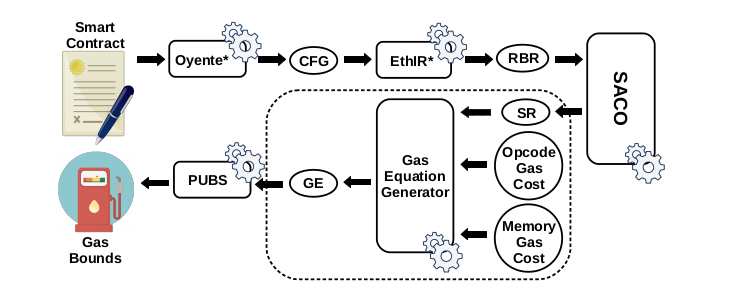
\includegraphics[scale=0.5]{GASTAP-structure.png}
        \caption[Struttura interna di GASTAP]{Architettura di GASTAP}
        \label{fig:gstp-struct}
    \end{figure}
    
    \begin{enumerate}
        \item \textbf{costruzione dei grafi control-flow (CFG)}: tale passaggio è realizzato con \textsc{oyente*}, un'estensione dell'omonimo tool \textsc{oyente} ~\cite{melonproject/oyente}.
        \item \textbf{decompilazione del codice di basso livello}: in questa fase il bytecode viene tradotto in una RBR (\textit{Rule-Based Representation}) grazie ad \textsc{ethir*}, estensione del già citato \textsc{ethir} ~\cite{albert2018ethir}.
        \item \textbf{deduzione delle relazioni di grandezza}: questo passaggio consiste nell'associare a ciascuna delle istruzioni in forma RBR le dimensioni dei dati con i quali interagisce. Quest'operazione è indispensabile per poter costruire le equazioni necessarie a calcolare i bound, e viene realizzata dal tool SACO ~\cite{10.1007/978-3-642-54862-8_46}, che produce le così dette SR (\textit{Size Relations}).
        \item \textbf{generazione delle equazioni di gas}: costituisce il core di GASTAP. Al fine di produrre le equazioni, il tool utilizza le SR insieme alla codifica dei costi delle istruzioni EVM, secondo le specifiche di \cite{wood2014ethereum}. Questi vengono suddivisi tra i costi richiesti dall'esecuzione del bytcode (\textit{Opcode Gas Cost}) e quelli richiesti per l'uso della memoria (\textit{Memory Gas Cost}). 
        \item \textbf{risoluzione delle equazioni fino a formare un bound}: per produrre il risultato finale GASTAP utilizza il solver PUBS ~\cite{albert2008automatic}, che risolve le GE (\textit{Gas Equations}) producendo una formula chiusa dei costi in termini di gas. 
    \end{enumerate}

    \subsection{Interfaccia Web}
    
    GASTAP è utilizzabile tramite un'interfaccia web, disponibile all'indirizzo \\
    https://costa.fdi.ucm.es/gastap.
    
    \begin{figure}[h]
        \centering
        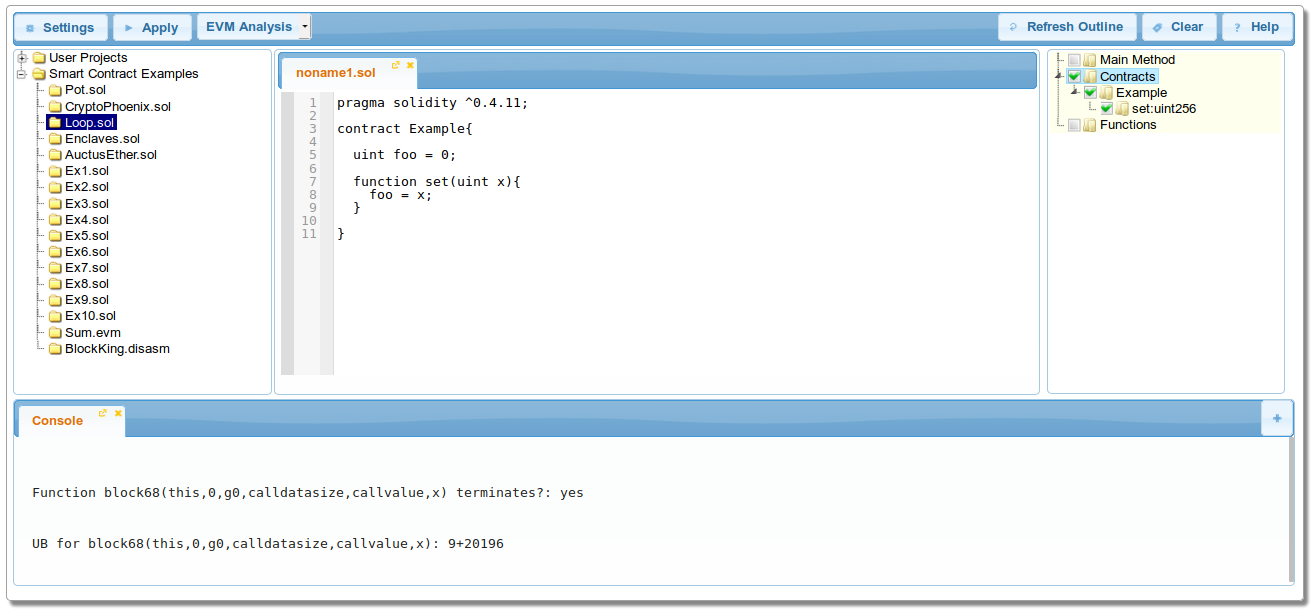
\includegraphics[scale=0.3]{GASTAP-example.png}
        \caption[Interfaccia di GASTAP]{Interfaccia di GASTAP}
        \label{fig:gstp-example}
    \end{figure}
    
    \`E possibile scrivere un proprio programma in Solidity oppure scegliere uno degli esempi proposti dal menù ``Smart Contract Examples''.\newline
    \indent Una volta selezionato il programma di input, cliccando su ``Refresh Outline'' GASTAP mappa le funzioni pubbliche del nostro programma, che vengono mostrate nella sezione di destra. Dopo aver selezionato i metodi che si vogliono analizzare, il pulsante ``Apply'' esegue l'analisi e produce un output nella Console.\newline
    \indent Nell'esempio viene proposto un semplice programma che setta una variabile globale. Stando all'output prodotto, tale programma è garantito teminare, e l'\textit{Upper Bound} (UB) ai consumi di gas è \verb|9+20196|. Si noti che l'upper bound fornito è sempre nella forma \textbf{memory bound} + \textbf{opcode bound}, dove le cifre si riferiscono rispettivamente al bound dei costi di memorizzazione e a quello dei costi delle operazioni che compongono il programma.\newline

    
    
\section{Compilatore solc}

Si tratta del compilatore ufficiale del linguaggio Solidity, utilizzabile da linea di comando.\newline
\indent Il comando \verb|solc --help| fornisce la spiegazione di ciascuna delle opzioni con cui può essere lanciato.

\lstset{
    style=cmd-line,
    literate={~} {$\sim$}{1}
}

\begin{lstlisting}
$~solc --help

solc, the Solidity commandline compiler.

This program comes with ABSOLUTELY NO WARRANTY. This is free software, and you
are welcome to redistribute it under certain conditions. See 'solc --license'
for details.

Usage: solc [options] [input_file...]

...

Allowed options:
  --help               Show help message and exit.
  --version            Show version and exit.
  --license            Show licensing information and exit.
    
...

  --gas                Print an estimate of the  
                       maximal gas usage for each 
                       function. 
 
\end{lstlisting}



Per condurre i nostri test abbiamo utilizzato il compilatore con l'opzione \verb|--gas|. In questa modalità il compilatore è in grado di determinare soltato dei bound costanti; in tutti gli altri casi produce \verb|infinite| come valore di output.\newline 
\indent Ecco un esempio del suo utilizzo sul programma raffigurato in figura \ref{fig:gstp-example}.

\begin{minipage}{\linewidth}
\begin{lstlisting}
$~solc --gas example.sol 

======= example.sol:Example =======
Gas estimation:
construction:
   5093 + 32800 = 37893
external:
   set(uint256):	20205

\end{lstlisting}
\end{minipage}


Confrontando i risultati ottenuti con quelli prodotti da GASTAP si evince che la stima del gas consumato dalla funzione \verb|set()| corrisponde a quela determinata da solc. Dunque l'uso dell'analisi statica non fa sì che si perda accuratezza nel calcolo.\newline
\indent Nella sezione 4.3.2 l'esempio verrà ripreso al fine di comprendere il bound.\newline


\newpage

\section{Test Condotti}

La nostra analisi è stata condotta su un insieme di programmi scritti in Solidity, disponibili nella repository ~\cite{melastone-sc}.\newline
\indent Ad eccezione del contratto \verb|four-function.sol|, proveniente dalla repository ~\cite{ethir-repository}, gli altri smart contract sono stati sviluppati seguendo la documentazione ufficiale del linguaggio Solidity ~\cite{solidity-docs}. Si tratta di semplici programmi ad hoc per il testing dei costrutti di base del linguaggio di programmazione. Di seguito i casi che abbiamo trattato.\newline

    
    \subsection{Operazioni di Assegnamento}
    
    I programmi \verb|assignment*.sol| implementano dei contratti che contengono un numero arbitrario di operazioni di assegnamento.
    
    \noindent
    \begin{minipage}[t]{.5\linewidth}
    \begin{lstlisting}
    //assignment2.sol
        
    pragma solidity ^0.4.11;

    contract B{

        function init(){
            uint number = 1;    
        }

    }

    \end{lstlisting}
    \end{minipage}
    \begin{minipage}[t]{.5\linewidth}
    \begin{lstlisting}
    //assignment4.sol

    pragma solidity ^0.4.11;

    contract D{

        uint foo;

        function reset(){
            uint foo = 0;    
        }

    }
    \end{lstlisting}
    \end{minipage}

    Abbiamo potuto verificare come l'operazione di assegnare un valore ad una variabile locale (\verb|assignment2.sol|) o globale (\verb|assignment3.sol|, \verb|assignment4.sol|) costa una quantità di gas relativamente bassa, in media 140 unità.
    Aggiungendo un'operazione di assegnamento in più, che va dunque ad incrementare il valore precedente della variabile, questa stima in alcuni casi subisce una crescita notevole: passiamo da 140 unità a circa 20000.
    
    \begin{center}
    \begin{minipage}{\linewidth}
    \begin{lstlisting}
    //assignment1.sol
        
    pragma solidity ^0.4.11;

    contract A{

        uint number = 0;

        function init(){
            number = 1;    
        }

    }
    \end{lstlisting} 
    \end{minipage}
    \end{center}

    
    Tale incremento è dato dalla presenza nel codice EVM dell'istruzione SSTORE (vedi Tabella \ref{tab:gas-costs}. Si evince dunque che la semplice operazione di settare il valore di una variabile da 0 ad uno diverso da 0 ha un impatto notevole sulla performance del programma in termini di costi. Un caso simile si era verificato nel caso del programma \verb|example.sol|.

    \subsection{Costrutto for}
    
    Testando i cicli for si è ottenuto un risultato interessante. La compilazione di questi programmi con solc produce sempre un bound infinito. Al contrario i test con GASTAP hanno prodotto una stima finita dei consumi. A titolo esemplificativo riportiamo di seguito i due esempi.
    
    \subsubsection{loop1.sol}
    
    \begin{minipage}{\linewidth}
    \begin{lstlisting}
    //loop1.sol
    //esegue la moltiplicazione
    //di number*a

    pragma solidity ^0.4.11;

    contract Loop1{

        uint sum = 0;
        uint number;
        
        function multiply(uint a){
            
            for(uint i = 0; i<a; i++){
            sum = sum+number;
            }
        }

    }
    \end{lstlisting}
    \end{minipage}

    Gli output ottenuti con solc e GASTAP sono, rispettivamente:
    
    \begin{minipage}{\linewidth}
    \begin{lstlisting}
    $~solc --gas loop1.sol
    
    ====== loop1.sol:Loop1 ======
    Gas estimation:
    construction:
    5099 + 39200 = 44299
    external:
    multiply(uint256):	infinite
    \end{lstlisting}
    \end{minipage}

    e \begin{lstlisting}
    GASTAP: 9+ (222+20476*nat(a))
    \end{lstlisting}

    
    
    \subsubsection{loop2.sol}
     
    \begin{minipage}{\linewidth}
    \begin{lstlisting}
    //loop2.sol
    //somma i primi 10 elementi di un vettore

    pragma solidity ^0.4.11;

    contract Loop2 {

        function sum (uint[] nums) returns (uint sol) {
            sol = 0;
            for(uint i = 0; i < 10; i++)
                    sol = sol+nums[i];
            }

    }
    \end{lstlisting}
    \end{minipage}

    
    Gli output ottenuti con solc e GASTAP sono, rispettivamente:
    
    \begin{minipage}{\linewidth}
    \begin{lstlisting}
    ======= loop2.sol:Loop2 =======
    Gas estimation:
    construction:
    111 + 59200 = 59311
    external:
    sum(uint256[]):	infinite
    \end{lstlisting}
    \end{minipage}

    
    e \begin{lstlisting} 
    GASTAP: 3*max([4+nat(nums)+1,4+nat(nums)+2])+pow(max([4+nat(nums)+1,4+nat(nums)+2]),2)/512+(1746+3* (1/32))
      \end{lstlisting}
    
    Come si può evincere da quest'ultimo caso gli upper bound forniti da GASTAP possono essere parametrici. Nell'esempio il parametro è determinato dal valore in input di una delle funzioni pubbliche del contratto.\newline
    \indent Più in generale possiamo dire che l'output prodotto da GASTAP è parametrico:
    \begin{itemize}
     \item nella dimensione dei parametri delle funzioni
     \item nello stato del contratto
     \item nei dati della blockchain dai quali dipendono i cosumi di gas (es. valore dell'ether)
    \end{itemize}


    
    \subsection{Cicli for Annidati}
    
    Per verificare la gestione dei cicli for annidati si è implementato un semplice programma che con il metodo \verb|suma(uint a)| esegue \verb|a| incrementi della variabile locale \verb|sum| attraverso un ciclo for.
    
    \begin{minipage}{\linewidth}
    \begin{lstlisting}
    //nested1.sol

    pragma solidity ^0.4.11;

    contract Nested1 {

        uint total_loops;

        // restituisce un valore uguale ad a, ottenuto sommando a volte 1.
        // ad ogni iterazione incrementa la var total_loops.
        function suma (uint a) returns (uint sum) {
            sum = 0;
            for(uint i = 0; i < a; i++)
                    sum = sum+1;
                    total_loops = total_loops +1;          
        }

    }
    \end{lstlisting}
    \end{minipage}

    
    Il programma è stato modificato in successione, inserendo un ciclo for annidato alla volta all'interno di \verb|suma(uint a)|. Ad ogni incremento abbiamo nuovamente calcolato il bound alla funzione \verb|suma(uint a)| con entrambi i programmi. Denotiamo con la variabile n il livello di annidamento dei cicli for. I risultati ottenuti sono mostrati nella Tabella \ref{tab:nested-outputs}.
    
    \begin{table}[h]
    \begin{threeparttable}[b]
     \begin{center}
        \caption[Analisi di nested*.sol]{Risultati dell'analisi dei contratti nested*.sol}\label{tab:nested-outputs}
        \begin{tabular}{ccp{12cm}}  
        \hline \hline   %inserisce due righe orizzontali
        $n$ & solc & GASTAP \\   %& separa le colonne
        \hline  %inserisce una riga orizzontale
        \bf1 & infinite & $15 + (20508+70*nat$\tnote{1}$(a))$\\
        \bf2 & infinite & $15 + (20548+70*nat(a)+20276*nat(a))$\\
        \bf3 & infinite & $15 + (20588+70*nat(a)+20276*nat(a)+20276*nat(a))$\\
        \bf4 & infinite & $15 + (20628+70*nat(a)+20276*nat(a)+20276*nat(a)+20276*nat(a))$\\
        \end{tabular}
        \begin{tablenotes}
            \item [1] La funzione nat è definita come nat(l)=max(0,l)
        \end{tablenotes}
     \end{center}
    \end{threeparttable}
    \end{table}

    
    Continuando ad incrementare il numero di cicli, si è potuto dare un bound al livello di annidamento. Per $n$ = 15 GASTAP non riesce a mappare le funzioni nella outline. Questo implica che non può essere condotta l'analisi sul programma \verb|nested15.sol|. Il limite dunque è dato dalla struttura del codice. L'esempio è mostrato in Figura \ref{fig:gstp-nested15}\newline
    
    \begin{figure}[h]
        \centering
        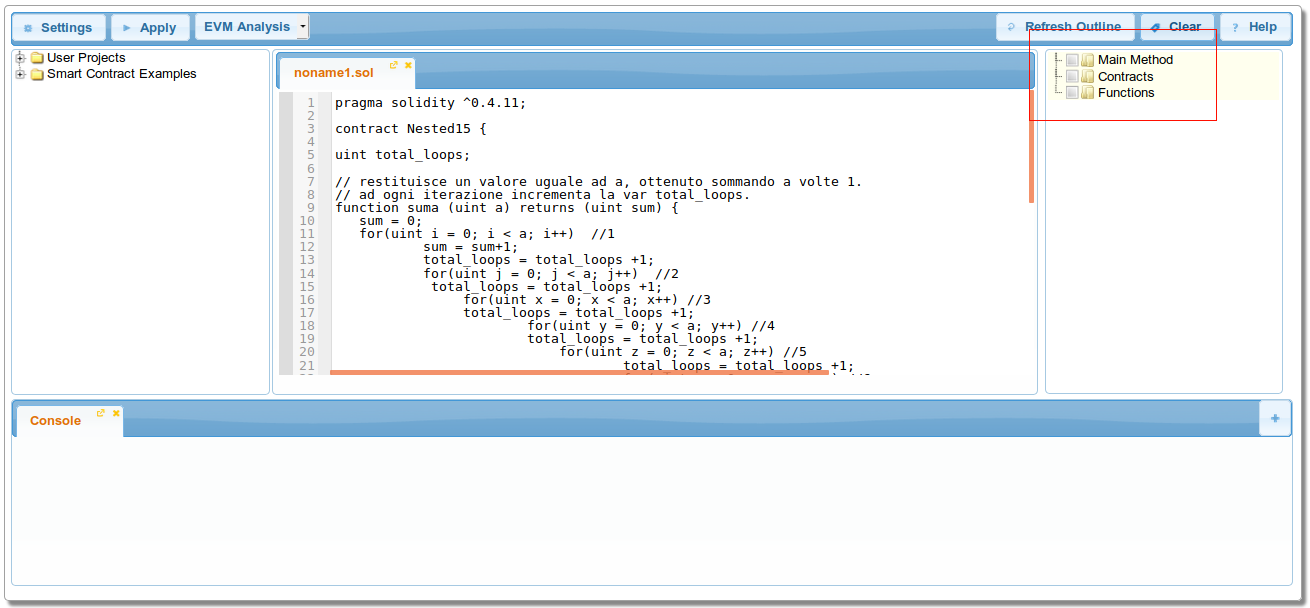
\includegraphics[scale=0.3]{GASTAP-nested15.png}
        \caption{nested15.sol in GASTAP}
        \label{fig:gstp-nested15}
    \end{figure}

    \begin{minipage}{\linewidth}
    \indent Dai risultati ottenuti conducendo i nostri test è stato possibile ricavare la seguente formula di ricorrenza per il bound determinato da GASTAP per i programmi nested$n$.sol:
    \[ \forall 0 < n \leq 14 \quad \mathrm{UB} = 15 + (20508 + (n - 1)*40 + 70*nat(a) + (n - 1)*20276*nat(a)) \]
    \end{minipage}

    \subsection{Costrutto while}
    
    Nel testare il comportamento dei tool di analisi di fronte a contratti contenenti dei cicli while abbiamo preso come input i file \verb|while1.sol| e \verb|while2.sol|.\newline
    
    \subsubsection{while1.sol}
    
    \indent Il primo programma implementa un algoritmo molto simile a quello di \verb|nested1.sol|. Abbiamo sostituito il ciclo for con un while, dunque il numero di iterazioni è facilmente determinabile, poichè equivalente al valore del parametro \verb|a|. Come nel caso dei cicli for solc produce un output infinito. Il risultato di GASTAP rispecchia un comportamento simile al caso precedente: viene determinato un bound parametrico in \verb|a|.\newline
    
    \begin{minipage}{\linewidth}
    \begin{lstlisting}
    //while1.sol

    pragma solidity ^0.4.11;

    contract A{

        uint number = 0;

        function init(uint a){
            
            while (a > 0) {
                number = number + 1;
                a = a - 1;
            }
        }

    }
    \end{lstlisting}
    \end{minipage}
    
    \begin{minipage}{\linewidth}
    \begin{lstlisting}
    ======= while1.sol:A =======
    Gas estimation:
    construction:
    5093 + 37600 = 42693
    external:
    init(uint256):	infinite
    \end{lstlisting}
    \end{minipage}

    
    e
    
    \verb|GASTAP: 9+ (209+20271*nat(a))|
    
    \subsubsection{while2.sol}
    
    Un caso differente si ha con il programma \verb|while2.sol|.
    Questo contratto implementa un algoritmo che calcola la radice quadrata del parametro in input \verb|x|. Anche in questo caso il bound dato da solc è infinito. Non solo GASTAP non riesce a determinare il bound - comportandosi quindi in modo simile a solc - ma addirittura va in errore.
    
    \begin{minipage}{\linewidth}
    \begin{lstlisting}
    //while2.sol

    pragma solidity ^0.4.11;

    contract B{

        function sqrt(uint x) returns (uint y) {
        
            uint z = (x + 1) / 2;
            y = x;
            
            while (z < y) {
                y = z;
                z = (x / z + z) / 2;
            }
        }
    }
    \end{lstlisting}
    \end{minipage}
    

    \begin{minipage}{\linewidth}
    \begin{lstlisting}
    ======= while2.sol:B =======
    Gas estimation:
    construction:
    99 + 48800 = 48899
    external:
    sqrt(uint256):	infinite
    \end{lstlisting}
    \end{minipage}

    
    e
    
    \verb|GASTAP: evm_solver:non_terminating|

    \newpage

    \subsection{Ricorsione}
    
    Per testare la ricorsione abbiamo utilizzato tre diversi programmi che implementano delle tecniche ricorsive diverse:
    \verb|ricorsione-diretta.sol|, \verb|ricorsione-indiretta.sol| e \verb|ricorsione-multipla.sol|. Per tutti e tre gli input entrambi i tool di analisi falliscono nel tentativo di stimare un bound. In base a questi risultati possiamo dunque asserire che i programmi ricorsivi non sono gestiti correttamente dai tool di analisi statica.\newline
    \indent Riportiamo di seguito il codice sorgente dei programmi utilizzati insieme ai risultati dell'analisi.\newline

        \subsubsection{Ricorsione Diretta}
        
        Questo programma contiene una sola funzione pubblica, \verb|fact(uint x)|. Questo metodo implementa l'algoritmo di calcolo del fattoriale di un numero. Consideriamo questo algoritmo ricorsivo \emph{diretto} in quanto la funzione fact richiama direttamente sé stessa.\newline
        
        \begin{minipage}{\linewidth}
        \begin{lstlisting}
        //ricorsione-diretta.sol

        pragma solidity ^0.4.19;

        contract Factorial{

            function fact(uint x) returns (uint y) {
                if (x == 0) {
                return 1;
                }
                else {
                return x*fact(x-1);
                }
            }
        }
        \end{lstlisting}
        \end{minipage}
        
        Gli output ottenuti con solc e GASTAP sono, rispettivamente:
        
        \begin{minipage}{\linewidth}
        \begin{lstlisting}
        ======= ricorsione-diretta.sol:Factorial =======
        Gas estimation:
        construction:
        93 + 42200 = 42293
        external:
        fact(uint256):	infinite
        \end{lstlisting}
        \end{minipage}

        e
    
        \begin{lstlisting}
        GASTAP: ../../bin/ethirweb   /tmp/ei_files0NMhje/noname1.sol  -entries  Factorial.fact:uint256 -type_file  solidity  > /dev/null ; cat /tmp/costabs/output.xml         
        \end{lstlisting}


        \subsubsection{Ricorsione Indiretta}
        
        Il seguente programma contiene uno schema di ricorsione \emph{indiretta}: il primo metodo, \verb|uno(uint n)| esegue una chiamata del secondo, \verb|due(uint n)|, che a sua volta richiama direttamente il primo.\newline
        
        \begin{minipage}{\linewidth}
        \begin{lstlisting}
        ​​//ricorsione-indiretta.sol

        pragma solidity ^0.4.19;

        contract ricorsione_indiretta {

            function uno(uint n) returns (uint m){
                if (n < 1) {
                    return 1;
                } 
                else {
                    return due(n - 1); // chiamata di due 
                }
            }

            function due(uint n) returns (uint m){
                if (n < 0) {
                    return 0;
                }
                else {
                    return uno(n/2); // chiamata di uno 
                }
            }
        }
        \end{lstlisting}
        \end{minipage}
        
        Gli output ottenuti con solc e GASTAP sono, rispettivamente:
        
        \begin{minipage}{\linewidth}
        \begin{lstlisting}
        ======= ricorsione-indiretta.sol:ricorsione_indiretta =======
        Gas estimation:
        construction:
        117 + 68600 = 68717
        external:
        due(uint256):	infinite
        uno(uint256):	infinite
        \end{lstlisting}
        \end{minipage}

        e
        \begin{minipage}{\linewidth}
        \begin{lstlisting}
        GASTAP: ../../bin/ethirweb   /tmp/ei_filesa6ppD5/noname1.sol  -entries  ricorsione_indiretta.uno:uint256 ricorsione_indiretta.due:uint256 -type_file  solidity  > /dev/null ; cat /tmp/costabs/output.xml         
        \end{lstlisting}
        \end{minipage}

        \subsubsection{Ricorsione Multipla}
        
        Il seguente programma contiene un metodo, \verb|fib(uint x)| che calcola il numero di Fibonacci del parametro \verb|x|. Tale metodo implementa una ricorsione \emph{multipla} in quanto contiene più chiamate a sé stesso.\newline
        
        \begin{minipage}{\linewidth}
        \begin{lstlisting}
        //ricorsione-multipla.sol

        pragma solidity ^0.4.19;

        contract Fibonacci {

            function fib(uint x) returns (uint y) {
            
                if (x == 1 || x == 2) {
                return 1;
                }
                
                else {
                return fib(x-1)+fib(x-2);
                }
            }
        }
        \end{lstlisting}
        \end{minipage}
        
        Gli output ottenuti con solc e GASTAP sono, rispettivamente:
        
        \begin{minipage}{\linewidth}
        \begin{lstlisting}
        ======= ricorsione-multipla.sol:Fibonacci =======
        Gas estimation:
        construction:
        99 + 46200 = 46299
        external:
        fib(uint256):	infinite
        \end{lstlisting}
        \end{minipage}

        e
    
        \begin{lstlisting}
        GASTAP: ../../bin/ethirweb   /tmp/ei_filesVQtMmj/noname1.sol  -entries  Fibonacci.fib:uint256 -type_file  solidity  > /dev/null ; cat /tmp/costabs/output.xml         
        \end{lstlisting}
        
     
    \newpage
     
    \subsection{Caso di studio: four-function.sol}
    
    Questo contratto contiene quattro funzioni pubbliche che si richiamano a vicenda. 
    
    \begin{minipage}{\linewidth}
    \begin{lstlisting}
    //four-function.sol

    pragma solidity ^0.4.11;

    contract Sum {

        function suma () returns (uint sol) {
            sol = 0;
            for(uint i = 0; i < 5; i++)
                    sol = sol+11;
            hola();
            adios(10);
        }

        function hola() {
            uint i = 0;
            i = i+15;
        }

        function adios(uint m) {
            uint c = 14;
            c = c+m;
            comer(c);   
        }

        function comer(uint x) {
            x = x*x;
            hola();
        }

    }
    \end{lstlisting}
    \end{minipage}
    
    La Tabella \ref{tab:four-function-outputs} mostra i risultati di solc e GASTAP a confronto. Nonostante il programma contenga delle chiamate ad altri metodi, si differenzia dal caso precedente dove era presente la ricorsione multipla. In questo caso non si verificano cicli nel grafo delle chiamate di funzione, dunque \verb|four-function.sol| non è ricorsivo.
    
    \begin{table}[h]
    \begin{center}
    \begin{tabular}{p{5cm}cp{6cm}}  
    \hline \hline
    \bf metodo & \bf solc & \bf GASTAP \\
    \hline
    adios(uint256) & 314 & 9+305\\
    comer(uint256) & 302 & 9+293\\
    hola() & 226 & 9+217\\
    suma() & infinite & 15+802\\
    \hline \hline
    \end{tabular}
    \caption[Analisi di four-function.sol]{Risultati dell'analisi del contratto four-function.sol}\label{tab:four-function-outputs}
    \end{center}
    \end{table}
    
    Ciò che emerge è che nel caso di bound costanti i risultati dei due tool sono uguali. \`E da notare il caso della funzione \verb|suma()|: solc non è in grado di produrre un bound. Questo è dovuto alla presenza del ciclo for all'interno del corpo della funzione, insieme alla chiamata della funzione \verb|adios()|. Rimuovendo le relative linee di codice riusciamo infatti ad ottenere un bound.\newline
    

        \noindent
    \begin{minipage}[t]{.5\linewidth}
    \begin{lstlisting}
    //four-function.sol:suma()
        
    function suma () returns (uint sol) {
        sol = 0;
        //for(uint i = 0; i < 5; i++)
        //        sol = sol+11;
        hola();
        //adios(10);
    }
    \end{lstlisting}
    \end{minipage}
    \begin{minipage}[t]{.5\linewidth}
    \begin{lstlisting}
    === four-functions.sol:Sum ===
    Gas estimation:
    construction:
    123 + 74600 = 74723
    external:
    adios(uint256):	314
    comer(uint256):	302
    hola():	226
    suma():	275
    \end{lstlisting}
    \end{minipage}




%%%%%%%%%%%%%%%%%%%%%%%%%%%%%%%%%%%%%%%%%non numera l'ultima pagina sinistra
\clearpage{\pagestyle{empty}\cleardoublepage}


%%%%%%%%%%%%%%%%%%%%%%%%%%%%%%%%%%%%%%%%%per fare le conclusioni
\chapter*{Conclusioni}

%imposta l'intestazione di pagina
\rhead[\fancyplain{}{\bfseries
CONCLUSIONI}]{\fancyplain{}{\bfseries\thepage}}
\lhead[\fancyplain{}{\bfseries\thepage}]{\fancyplain{}{\bfseries
CONCLUSIONI}}

%aggiunge la voce Conclusioni nell'indice
\addcontentsline{toc}{chapter}{Conclusioni}

L'utilizzo dell'analisi statica nella verifica delle proprietà di sicurezza dei contratti di Ethereum ha riscosso successo recentemente, portando allo sviluppo di alcuni software che combinano diverse tecniche di analisi statica. Solo una piccola porzione di questi programmi si focalizza sui consumi di gas; abbiamo visto \textsc{MadMax}~\cite{grech2018madmax}, che conduce un'analisi orientata a individuare vulnerabilità nel codice legate al gas. Un altro tool simile è \textsc{Gasper}~\cite{chen2017under}, che grazie all'analisi dei consumi è in grado di individuare dei pattern ai quali è associato un elevato consumo di gas; offre dunque un servizio di ottimizzazione del codice. Nessuno di questi però è in grado di produrre dei bound.\newline
\indent La stima dei consumi di gas resta quindi un topic poco trattato. I lavori condotti in questa direzione sono ancora pochi: oltre al tool \textsc{Gastap}~\cite{DBLP:journals/corr/abs-1811-10403}, sul quale ci siamo focalizzati durante questa trattazione, è importante citare anche il lavoro di Marescotti et al.~\cite{marescotti2018computing}, che sottolineando l'importanza del tema, propone due algoritmi per la stima dei consumi di gas; questo approccio tuttavia non è stato ancora implementato, motivo per cui non è stato possibile includerlo in questo lavoro.\newline
\indent Va inoltre considerato che questi strumenti hanno ancora molte limitazioni, impedendo la verifica di programmi sofisticati. Costrutti come i cili while o la ricorsione non vengono gestiti correttamente, ponendo una forte limitazione allo sviluppatore che desideri verificare i consumi del proprio programma. Per questa ragione l'impiego dell'analisi nel mondo reale non è ancora auspicabile, ma dati i suoi vantaggi e l'utilizzo sempre più diffuso della piattaforma Ethereum possiamo contare che la ricerca ci porti nella giusta direzione.\newline  


%imposta l'intestazione di pagina
%\renewcommand{\chaptermark}[1]{\markright{\thechapter \ #1}{}}
%\lhead[\fancyplain{}{\bfseries\thepage}]{\fancyplain{}{\bfseries\rightmark}}

%%%%%%%%%%%%%%%%%%%%%%%%%%%%%%%%%%%%%%%%%non numera l'ultima pagina sinistra
\clearpage{\pagestyle{empty}\cleardoublepage}

%\appendix                               %imposta le appendici

%\chapter{Prima Appendice}               %crea l'appendice
%In questa Appendice non si \`e utilizzato il comando:\\
%%%%%%%%%%%%%%%%%%%%%%%%%%%%%%%%%%%%%%%%%\verb"" � equivalente all'
                                        %   ambiente verbatim,
                                        %   ma si utilizza all'interno
                                        %   di un discorso.
%\verb"\clearpage{\pagestyle{empty}\cleardoublepage}", ed infatti
%l'ultima pagina 8 ha l'intestazione con il numero di pagina in
%alto.

%%%%%%%%%%%%%%%%%%%%%%%%%%%%%%%%%%%%%%%%%imposta l'intestazione di pagina
%\rhead[\fancyplain{}{\bfseries \thechapter \:Prima Appendice}]
%{\fancyplain{}{\bfseries\thepage}}


%\chapter{Seconda Appendice}             %crea l'appendice

%%%%%%%%%%%%%%%%%%%%%%%%%%%%%%%%%%%%%%%%%imposta l'intestazione di pagina
%\rhead[\fancyplain{}{\bfseries \thechapter \:Seconda Appendice}]
%{\fancyplain{}{\bfseries\thepage}}


\rhead[\fancyplain{}{\leftmark}]{\fancyplain{}{\thepage}}
\lhead[\fancyplain{}{\thepage}]{\fancyplain{}{\rightmark}}

%aggiunge la voce Bibliografia nell'indice
\addcontentsline{toc}{chapter}{Bibliografia}

\bibliography{bibliografia}{}
\bibliographystyle{plain}


%%%%%%%%%%%%%%%%%%%%%%%%%%%%%%%%%%%%%%%%%non numera l'ultima pagina sinistra
\clearpage{\pagestyle{empty}\cleardoublepage}

%\chapter*{Ringraziamenti}
%\thispagestyle{empty}
%Qui possiamo ringraziare il mondo intero!!!!!!!!!!\\
%Ovviamente solo se uno vuole, non \`e obbligatorio.

\end{document}
